\chapter*{Wstęp}
Często głównym zadaniem tworzonego oprogramowania jest prezentacja pewnych danych. Nawet najlepszy program wykonujący skomplikowane obliczenia jest niewiele wart dla klienta, jeśli nie potrafi w~przystępny sposób zaprezentować efektów swoich działań. Ważnym tematem jest również dostosowanie sposobu prezentacji do odbiorcy.
 
Podstawową formą prezentacji danych w~informatyce i~nie tylko są tabelki. Jest to forma umożliwiające wyświetlanie danych bardzo precyzyjnych. Qt posiada już architekturę służącą tworzeniu takich systemów -- Model-Widok-Delegat. Jest to bardzo popularna platforma umożliwiająca tworzenie kilku rodzajów widoków prezentujących dane z~różnych źródeł.

Wykresy są graficzną formą prezentacji danych, która jest równie popularna co tabelki. Jest to forma może mniej precyzyjna, ale dużo bardzo przystępna dla ludzkiej percepcji. Wykresy ułatwiają szybkie porównywanie wielu rekordów oraz wyznaczanie tendencji. Ponadto jej graficzna oraz możliwe animacje sprawiają, że jest ona bardzo atrakcyjna dla końcowego użytkownika oprogramowania.

Qt posiada już kilka bibliotek służących tworzeniu wykresów, jednak, jak wynika z~rozdziału \textit{Przegląd dziedziny}, nadal istnieje zapotrzebowanie na wartościowe rozwiązanie open-source.

Na początku tej pracy omawiam dostępne biblioteki do tworzenia wykresów w~Qt. Następnie przedstawiam opis i~analizę wymagań stawianych mojej bibliotece. Kolejny rozdział to projekt architektury całej biblioteki, wykonany z~pomocą diagramów UML. Następne dwa rozdziały są poświęcone implementacji oraz testom biblioteki. Ostatni rozdział zawiera wnioski dotyczące stworzonej biblioteki oraz możliwości jej dalszego rozwoju. 

\chapter{Wprowadzenie}
\section{Qt}
Qt jest zbiorem bibliotek języka C++, które najczęściej są rozpowszechniane jako biblioteki dynamiczne. Źródła Qt są dostępne na stronie właściciela -- firmy Digia~\footnote{\url{http://qt.digia.com}}. Lista bibliotek jest dość okazała, a~znaleźć na niej można narzędzia do tworzenia interfejsów użytkownika, parsowania plików XML czy dostępu do baz danych. Podstawowym celem twórców Qt było stworzenie przenośnych, wygodnych dla programisty oraz wydajnie działających bibliotek. Przenośność pomiędzy najpopularniejszymi platformami, osiągnięto na poziomie kodu źródłowego. Naczelną zasadą Qt jest: \textit{pisz raz, kompiluj wielokrotnie}. 

\begin{figure}
\centering
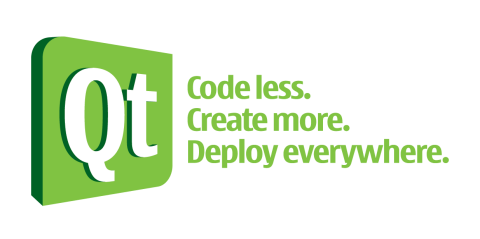
\includegraphics[scale=0.7]{img/qt-rule.png}
\caption{Motto Qt}
\end{figure}

\subsection{Narzędzia}
Najważniejszymi narzędziami, które umożliwiają tudzież ułatwiają pracę z~Qt są:
\begin{itemize}
\item moc (Meta Object Compiler) -- specjalny program, który można porównać do preprocesora. Na podstawie naszego kodu generuje on dodatkowe pliki źródłowe potrzebne Qt, bedące niewidocznymi dla programisty.
\item uic (User Interface Compiler) -- kompilator plików *.ui, które zawierają informację o~układzie interfejsu użytkowniak.
\item qmake -- program, który na podstawie pliku projektu tworzy plik Makefile. Ułatwia w~znaczny sposób zarządzanie procesem budowania.
\item Qt Creator -- zintergrowane środowisko programistyczne, przeznaczone głównie dla języków C++ i~JavaScript.
\item Qt Designer -- program umożliwiający łatwe tworzenie interfejsów użytkownika. Generuje on wspomniane juz pliki *.ui.
\end{itemize}


\subsection{QObject}
C++ nie wymusza dziedziczenia po określonej klasie, jak ma to miejsce chociażby w~Javie, gdzie zawsze na szczycie drzewa dziedziczenia znajduje się klasa \textit{Object}. Korzystając z tej niszy, Qt wprowadza swoją klasę -- \textit{QObject}. Dzięki wielodziedziczeniu, nie musimy rezygnować z dotychczasowej hierarchii dziedziczenia, aby otrzymać wiele ciekawych możliwości płynących z~wykorzystania \textit{QObject}.
Niektóre z~nich to:
\begin{itemize}
\item Relacja rodzic--dziecko, która jest nawiązywana w chwili tworzenia obiektów. Umożliwia ona wyszukiwanie dzieci danego obiektu po ich klasie, bądź nazwie. Ponadto ułatwia zarządzanie pamięcią, poprzez automatyczne usuwanie obiektów -- dzieci w chwili usunięcia rodzica. Przykład: usunięcie okna zawierającego wiele elementów spowoduje posprzątanie ze sterty wszystkich przycisków, etykiet czy obrazków.
\item \textit{qobject\_cast} -- dynamiczne rzutowanie, stosowane zazwyczaj do rzutowania w dół hierarchii dziedziczenia. Jest ono znacznie szybsze od \textit{dynamic\_cast}, gdyż nie korzysta z mechanizmu RTTI (Run Time Type Information). Jedynym oczywistym mankamentem jest fakt, że rzutowanie to działa jedynie dla klas dziedziczących po \textit{QObject}.
\item Zdarzenia -- niskopoziomowy mechanizm komunikacji. Qt opakowuje standardowe zdarzenia w obiekty swoich klas i~dostarcza je do odpowiednich obiektów. Przed dostarczeniem zdarzenia do adresata można je przefiltrować, podejrzeć lub wręcz zmienić.
\item Sygnały i~sloty -- wysokopoziomowy mechanizm komunikacji będący implementacją wzorca \textit{Obserwator}.
Jest to bardzo wygodny sposób na luźne wiązanie obiektów, które mogą ze sobą współpracować, nie wiedząc nawzajem o swoim istnieniu.
\item Właściwości -- sposób na parametryzowanie obiektów. Istnieją zarówno właściwości statyczne, dodawane w czasie kompilacji, wspólne dla wszystkich obiektów danej klasy, np. wysokośc czy kolor, jak i~dynamiczne, przypisywane pojedynczym obiektom już w czasie wykonania programu.
\end{itemize}

\section{Qt Quick}
Qt~Quick~\footnote{\url{http://qt.digia.com/Product/qt-quick}} jest nową technologią tworzenia GUI. Jej przeznaczeniem jest tworzenie lekkich, intuicyjnych oraz płynnie działających interfejsów, głównie na platformach mobilnych. W przeciwieństwie do tradycyjnego Qt, Qt~Quick nie wymaga znajomości C++, co ma dopuścić do pracy nad GUI nie tylko programistów, ale również projektantów -- grafików.
Na Qt~Quick składają się:
\begin{itemize}
\item QML -- deklaratywny język,
\item JavaScript -- imperatywny język,
\item Środowisko uruchomieniowe zintegrowane z Qt,
\item Designer,
\item API C++ umożliwiające integrację z aplikacjami Qt.
\end{itemize}

W Qt4, Qt~Quick był oparty na architekturze \textit{Graphics View}~\footnote{Framework Graphics View\url{http://qt-project.org/doc/qt-5.0/qtwidgets/graphicsview.html}}, jednak problemy wydajnościowe zmusiły projektantów do sięgnięcia po bardziej zaawansowane narzędzia. W Qt5 wykorzystano bezpośrednio \textit{OpenGL} oraz \textit{SceneGraph}~\footnote{Scene Graph\url{http://en.wikipedia.org/wiki/Scene\_graph}}. Ponadto w celach optymalizacyjnych zrezygnowano z~własnego silnika języka JavaScript i skorzystano z gotowego rozwiązania -- \textit{Google~V8}.

\subsection{QML}
QML (Qt Modeling Language) jest deklaratywnym językiem służącym głównie do opisu wyglądu i~zachowania GUI. QML może jednak służyć do zupełnie innych zastosowań. W~nowy systemie zarządzania procesem budowania projektów napisanych w~Qt -- QBS~\footnote{Qt Build Suit \url{http://qt-project.org/wiki/qbs}}, językiem opisu projektu jest właśnie QML.\newline

Relacja rodzic-dziecko elementów QML została zorganizowana w~drzewiastą strukturę, ułatwiającą zarządzanie elementami. Podobnie jak obiekty w~klasycznym Qt, elementy posiadają szereg właściwości, np. id lub szerokość. W~QML wartość nie jest przypisywana właściwości, a~jest z nią wiązana, dzięki czemu właściwość ta może być stale aktualizowana.\newline

Elementy QML mogą być rozszerzane przez kod napisany w~JavaScript lub poprzez integrację z modułami napisanymi w~C++.

\subsection{Przykładowy kod QML}

\begin{verbatim}
Item {
width: 400; height: 200
   Rectangle {
   id: rect
   x: 100; y: 50;
   width: height / 2; height: parent.height
   anchors.centerIn: parent
   color: "lightblue"
   }
}
\end{verbatim}

Wykonanie powyższego kod spowoduje wyświetlenie okienka z~rysunku~\ref{rys:qml}. Główny element interfejsu jest typu \textit{Item} i~ma wymiary 400x200 pikseli. Posiada on dziecko będące prostokątem o~tej samej wysokości i~szerokości równej połowie jego wysokości. Ponadto prostokąt ten jest wyśrodkowany w~swoim rodzicu oraz ma jasnoniebieski kolor.

Jak widać dziecko może odwoływać się do swego rodzica za pomocą słowa \textit{parent}. Z~kolei inne elementy mogą się odwoływać do danego elementu za pomocą jego właściwości -- id.

\begin{figure}
\centering
\caption{Przykład wykorzystania QML}\label{rys:qml}
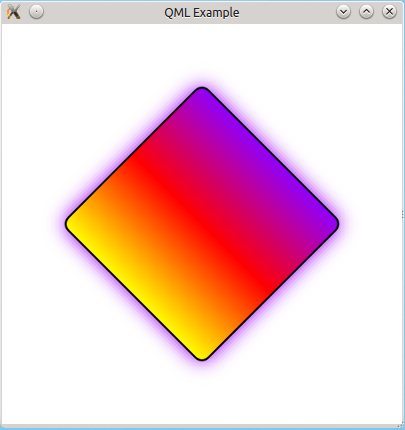
\includegraphics[scale=0.8]{img/qml.png}
\end{figure}

